\chapter{State of the Art}%
\label{chapter:State of the Art}

\begin{introduction}
This chapter will provide a comprehensive review of current \ac{5G} and Wi-Fi integration efforts, existing authentication mechanisms, and challenges in device identification. It will also explore recent developments and proposed solutions in the field, setting the context for our research.
\end{introduction}

\section{Why \acs{4G} needed improved security?}

From the point of view of authentication, a cellular network consists of three main components: User Equipment (UE), a Serving Network (SN), and a Home Network (HN).

The UE refers to devices like smartphones, tablets, or IoT devices equipped with a UICC  hosting at least a Universal Subscriber Identity Module (USIM) storing a cryptographic key that is shared with the subscriber’s home network. These devices connect to the network over radio signals. In 4G networks, these signals are based on technologies like LTE (Long-Term Evolution), utilizing frequency bands allocated for mobile communication.

The Serving Network (SN) includes network components that facilitate communication and provide services to the UE in a specific geographic area. Key elements of the SN are the eNodeB (Evolved Node B) and the MME (Mobility Management Entity).

\begin{itemize}
    \item{
        The eNodeB is a base station that manages the radio connection between the UE and the network. It handles tasks like scheduling radio resources, modulating and demodulating signals, and ensuring reliable data transmission over the air interface.
    }
    \item {
        The MME is a core network element responsible for managing signaling between the UE and the core network. It plays a key role in tasks such as authenticating the user, establishing bearers (data pathways), and ensuring mobility by managing handovers between eNodeBs as the UE moves.
    }
\end{itemize}

The Home Network (HN) refers to the network operated by the user's mobile service provider (e.g., MEO, Vodafone, or NOS). It stores subscriber information in a database called the Home Subscriber Server (HSS).

\begin{itemize}
    \item {
        The HSS is a critical component that contains user-specific data, such as subscription profiles, service entitlements, and cryptographic keys. These keys are used during the authentication process to verify that the user is authorized to access the network. The HSS communicates with the SN to authenticate the UE using protocols like Diameter over an IP-based system. This ensures secure and efficient exchange of authentication and session-related information.
    }
\end{itemize}

Communication between the SN and HN over the IP network is facilitated by core network protocols. The SN sends a request to the HSS containing the UE’s credentials (e.g., IMSI, International Mobile Subscriber Identity). The HSS uses its stored keys to generate authentication vectors, which are then sent back to the SN. The SN uses these vectors to authenticate the UE and establish a secure connection.

Together, these components form the Evolved Packet System (EPS)~\cite{cbl-comp-4g-5g-p3}, the architecture underlying 4G LTE networks. The EPS enables seamless connectivity and service delivery by integrating the radio access network (eNodeBs) with the core network components (e.g., MME and HSS). This design ensures that authentication, data management, and mobility are handled efficiently while providing high-speed, low-latency connections for the UE.

Prior generations to 4G, especially in Radio Access Networks (RANs), have faced significant security and privacy challenges. One major issue was the lack of network authentication in 2G, which allowed attackers to perform network spoofing using fake base stations. For example, a fake base station could advertise a stronger signal and lure User Equipment (UE) away from its legitimate network, enabling the attacker to send fraudulent text messages to the user.

Another issue was the lack of integrity protection for signaling messages, which left them vulnerable to spoofing and tampering. For instance, fake base stations could send unprotected Identity Request messages (a Non-Access Stratum [NAS] signaling message in LTE) to steal permanent UE identifiers, such as the IMSI.

Additionally, certain messages lacked confidentiality, resulting in privacy violations. For example, unencrypted paging messages could be intercepted to detect a user’s presence and track their precise location. 

To mitigate these vulnerabilities, the 3GPP introduced the Authentication and Key Agreement (AKA) protocol, which ensures entity authentication, message integrity, and message confidentiality. AKA employs a challenge-response mechanism based on a symmetric key shared between the subscriber and their home network. It also derives cryptographic keying materials to protect both signaling messages and user plane data, including communications over radio channels. This protocol significantly enhances security and privacy in mobile networks.

In 4G EPS-AKA, despite the enhancements brought by the 3GPP AKA protocol, two significant flaws remain. First, during the initial stage of the authentication process (the flow is shown in Figure \ref{fig:4g-authentication-procedure}), the User Equipment (UE) must transmit its identity, specifically its IMSI, to the serving network. This identity is sent over the radio network without encryption, leaving it vulnerable to interception~\cite{cbl-comp-4g-5g-p3}. Although the use of a temporary identifier, such as the Globally Unique Temporary Identifier (GUTI), is intended to mitigate this risk, researchers have demonstrated that GUTI allocation is flawed in that the identifiers either do not change frequently enough~\cite{gt-freq} or are assigned in predictable patterns~\cite{gt-pred}.

Second, during the authentication decision, the home network may provide an Authentication Vector (AV), but this value is not directly included in the decision-making process, which is handled solely by the serving network~\cite{cbl-comp-4g-5g-p4}.

\begin{figure}[htbp]
    \centering
    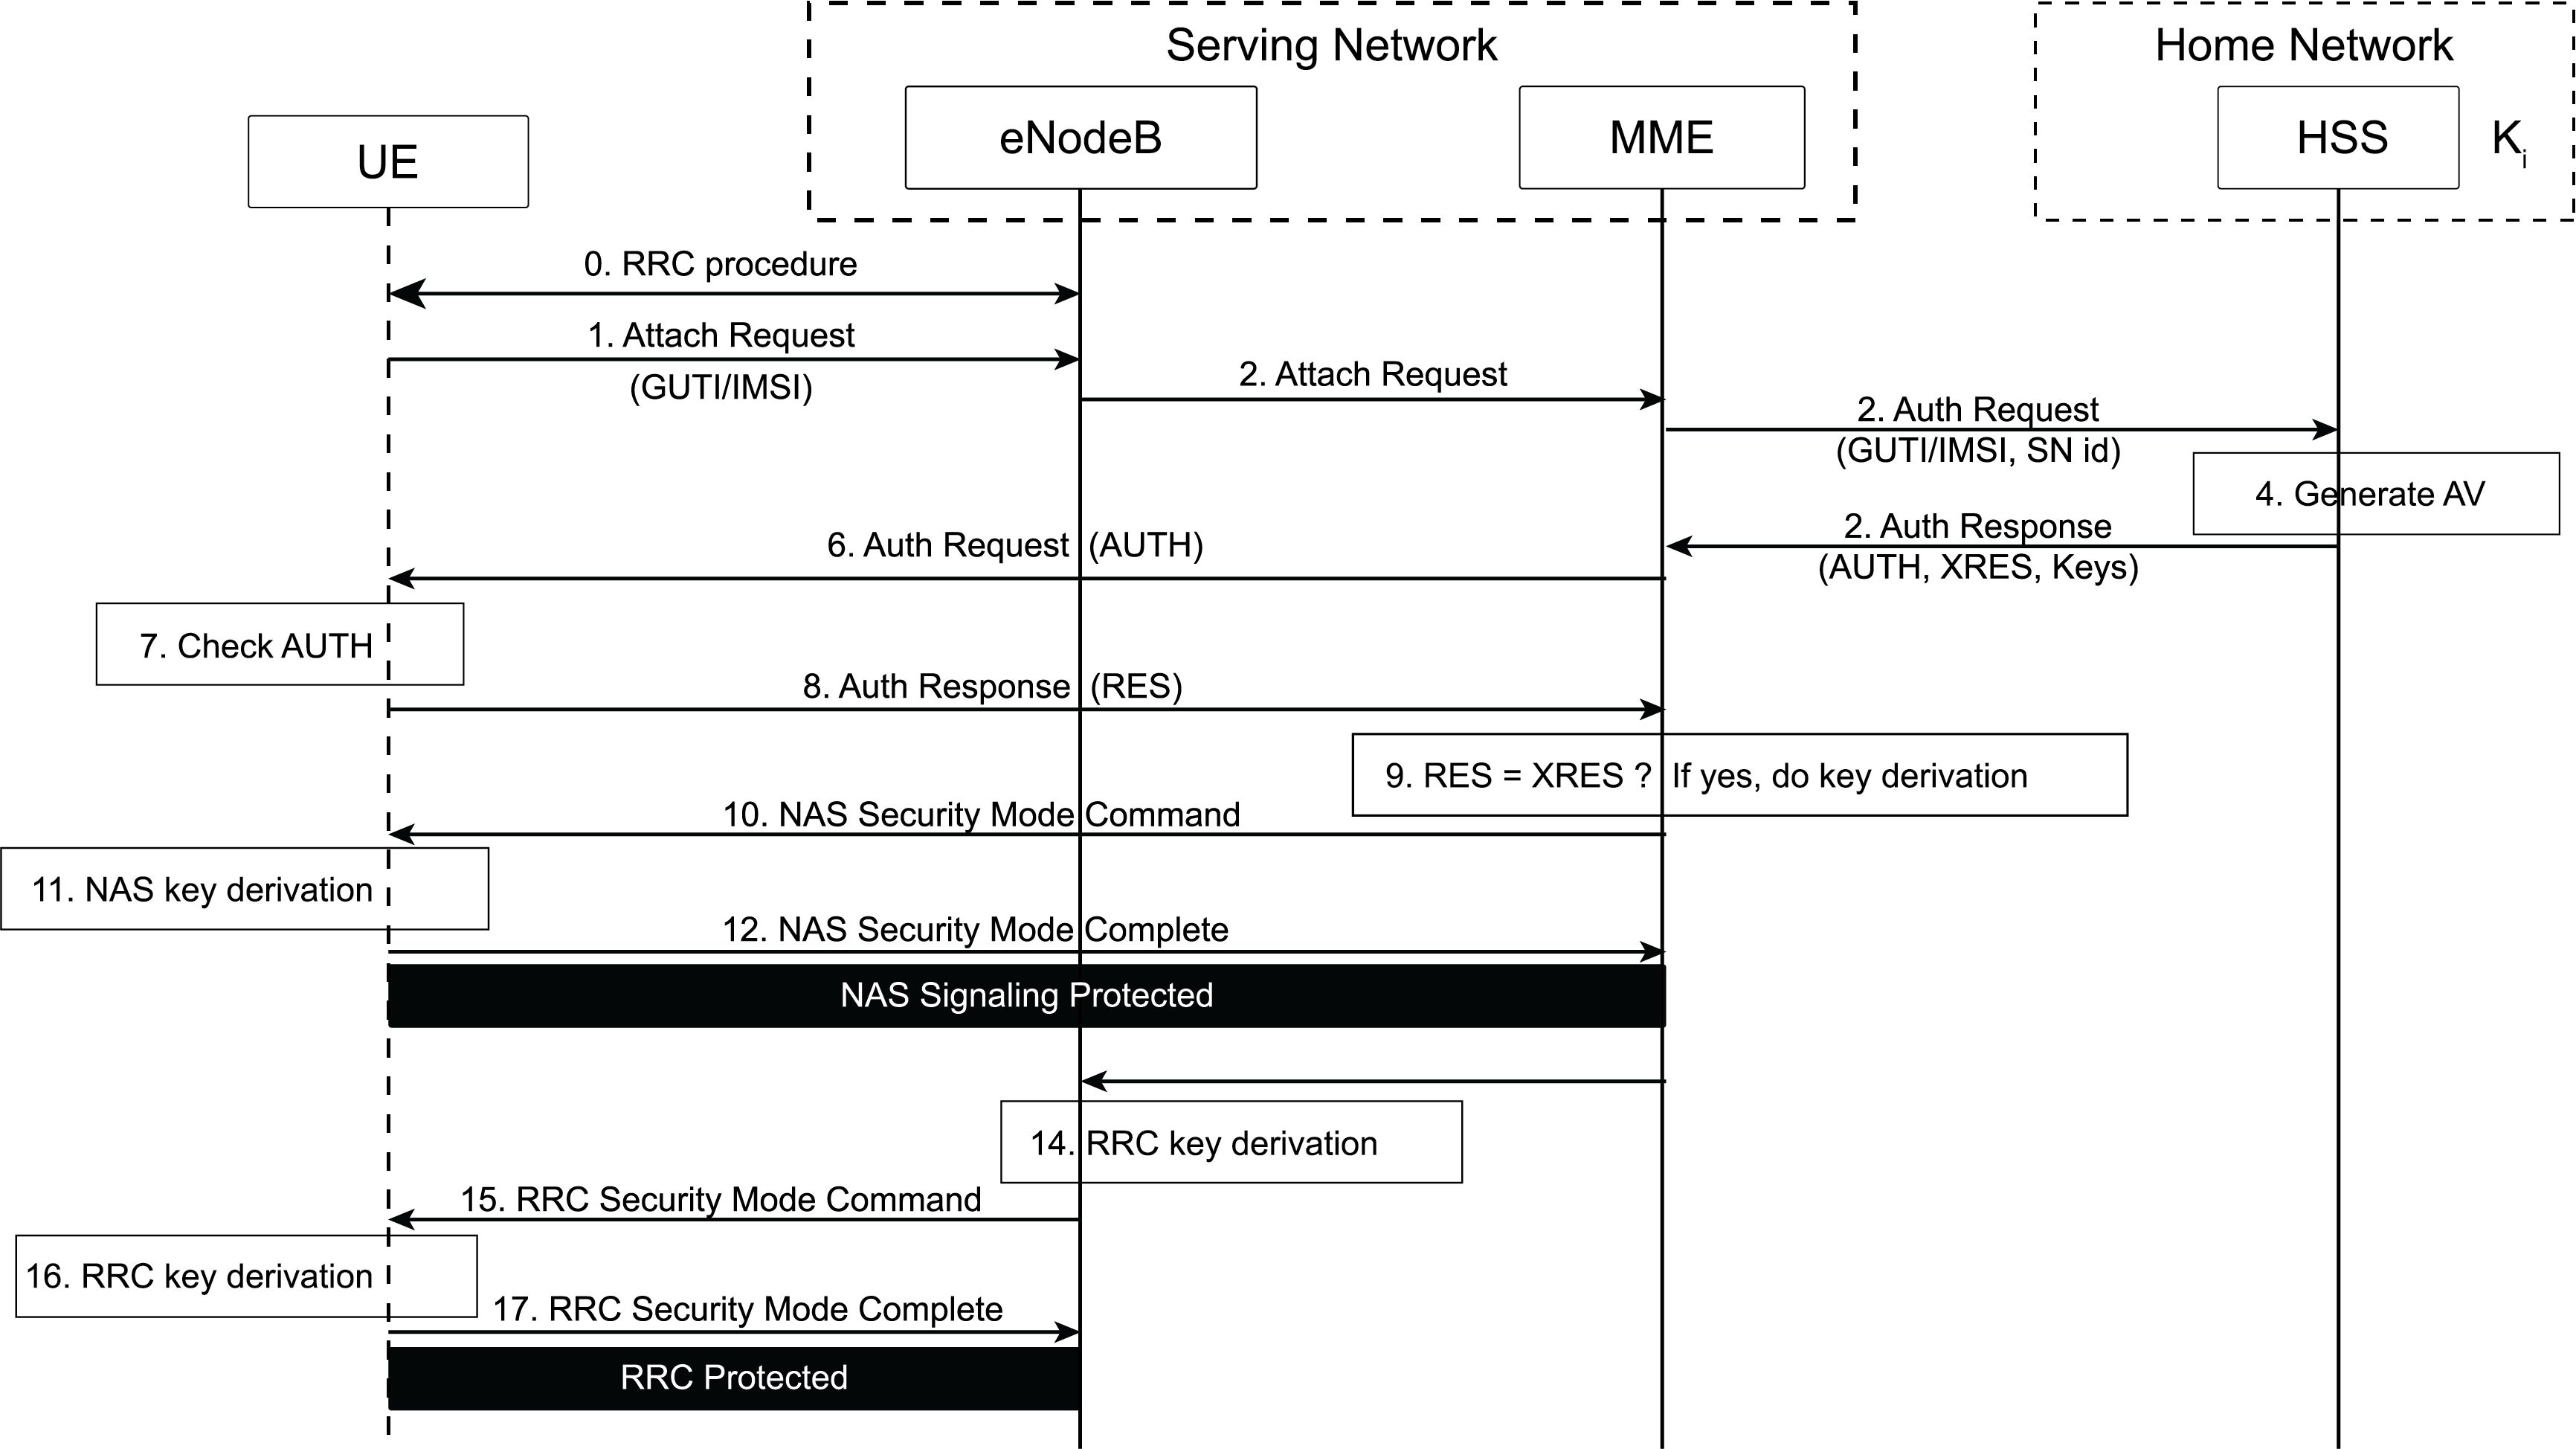
\includegraphics[width=0.75\textwidth]{figs/4g-authentication-procedure.png}
    \caption{\ac{4G} Authentication Procedure}
    \label{fig:4g-authentication-procedure}
\end{figure}

\section{\acs{5G} Architecture and Security Framework}

The 5G System architecture, seen in Figure \ref{fig:5g-system-architecture}, is designed to support advanced techniques such as Network Function Virtualization (NFV) and Software-Defined Networking (SDN). It separates Control Plane (CP) and User Plane (UP) functions, enabling independent scalability, evolution, and flexible deployments in centralized or distributed locations. The architecture uses modular function design to support efficient network slicing and defines procedures as reusable services to enhance flexibility. It minimizes dependencies between the Access Network (AN) and the Core Network (CN) by integrating different access types, including 3GPP and non-3GPP, through a converged core network.

\begin{figure}
    \centering
    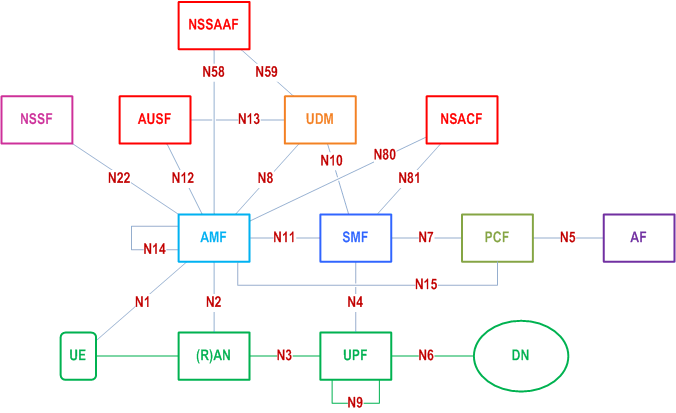
\includegraphics[width=0.75\linewidth]{figs/5g-system-architecture.png}
    \caption{5G System Architecture}
    \label{fig:5g-system-architecture}
\end{figure}

The system includes a unified authentication framework, supports stateless Network Functions (NFs) by decoupling compute and storage resources, and enables capability exposure for network features. It allows concurrent access to local and centralized services and deploys UP functions near the Access Network to support low latency services and local data network access. Additionally, it supports roaming with both home-routed and local breakout traffic in visited networks, ensuring efficient and flexible operation.%cite 23.501 4.1

In 5G, the security framework is built around a new way of organizing the network, known as Service-Based Architecture (SBA). This setup introduces new entities and processes that focus on keeping the network secure, especially when it comes to authentication, which is the process of verifying users and devices.

% cite 23.501 6.2.X for each
\begin{itemize}
    \item{
        One of the key entities is the Security Anchor Function (SEAF), located in the serving network. Acrting as an intermediary during the authentication process. The SEAF receives authentication requests from a device (UE), but it relies on the home network to decide whether the authentication is valid or not. It can reject the authentication, but the final decision rests with the home network.
    }
    \item{
        The Authentication Server Function (AUSF) is the entity in the home network that actually decides whether the device should be allowed onto the network. The AUSF looks at the information provided by the device and checks it against the home network's security policies. It then works with other backend services to compute the necessary data and keys needed to authenticate the device, using secure methods like 5G-AKA or EAP-AKA’.
    }
    \item{
        The Unified Data Management (UDM) is in charge of managing the data involved in authentication. One of its key roles is managing the Authentication Credential Repository and Processing Function (ARPF), which selects the right authentication method based on the device's identity and the network's policies. It also helps generate the keys and data that the AUSF uses for authentication.
    }
    \item{
        Finally, the Subscription Identifier De-concealing Function (SIDF) helps protect the subscriber's permanent identity (called the SUPI). In 5G, this permanent identity, which could be something like a user’s IMSI, is always kept hidden and encrypted when sent over the air to prevent hackers from tracking it. The SIDF is the only part of the network that can decrypt the encrypted identity (called the SUCI) using a private key, ensuring that no one else can access the user’s personal details.
    }
\end{itemize}

At its core, this framework introduces a unified and flexible authentication system that seamlessly integrates both 3GPP (traditional cellular) and non-3GPP (such as Wi-Fi or cable) networks. This cross-network compatibility is crucial for enabling a wide range of access methods and supporting the growing ecosystem of connected devices.

Central to this framework is the Extensible Authentication Protocol (EAP), which facilitates secure communication between the User Equipment (UE) and the Authentication Server Function (AUSF). The Security Anchor Function (SEAF) acts as an intermediary, relaying authentication messages between the UE and AUSF. This setup supports various authentication methods, including 5G-AKA, EAP-AKA', and EAP-TLS, providing robust security for data exchange. For untrusted non-3GPP access, the Non-3GPP Interworking Function (N3IWF) comes into play, establishing a secure IPsec tunnel between the UE and the 5G core network, ensuring encrypted communication even over potentially insecure networks.%cite 23.501 6.2.x for NF

A key innovation in the 5G authentication framework is its ability to establish multiple security contexts during a single authentication process. This feature allows users to transition seamlessly between different network types without the need for re-authentication, significantly enhancing user experience and maintaining continuous secure access. Furthermore, the framework introduces improved subscriber privacy through the use of concealed subscriber identities (SUCI), protecting users from potential tracking or interception of their permanent identities (SUPI).%First part needs citation

\subsection{Comparing \acs{5G-AKA}, \ac{EAP-AKA'} and \ac{EAP-TLS}}

The 5G-AKA authentication process begins when the Security Anchor Function (SEAF) receives a request from the User Equipment (UE) seeking network access. The UE provides either a 5G-GUTI (Globally Unique Temporary Identifier) or a SUCI (Subscription Concealed Identifier) to begin the authentication. The AUSF (Authentication Server Function) first ensures that the requesting network is legitimate, then it sends an authentication request to the UDM/ARPF (Unified Data Management/Authentication Credential Repository and Processing Function). If the SUCI is provided, the SIDF (Subscription Identifier De-concealing Function) decrypts it to obtain the SUPI (Subscription Permanent Identifier), which is used to determine the authentication method.%cite 33.501 or 23.501

% add image of 5G-AKA flow

Next, the UDM/ARPF generates an authentication response containing tokens and keys. These are sent to the AUSF, which computes a hash (HXRES) and checks the expected response. The AUSF sends the authentication result, including the AUTH token and HXRES, to the SEAF, ensuring that the SUPI is not exposed to the SEAF, preserving privacy. The SEAF forwards the AUTH token to the UE, which then validates it using a secret key shared with the home network. If successful, the UE computes a RES token and sends it back to the SEAF. The SEAF forwards this to the AUSF, which validates the response.

Once the RES token is verified, the AUSF sends an anchor key to the SEAF. The SEAF derives an AMF key, which the AMF (Access and Mobility Management Function) uses to generate further keys for securing signaling messages between the UE and network elements. The UE, using its root key, can derive all necessary keys for secure communication with the network, ensuring mutual trust and security.

% add image of EAP-AKA' flow

% add image of NAS message structure

An alternative authentication method in 5G is EAP-AKA', which provides mutual authentication between the UE and the network using a shared cryptographic key. Unlike 5G-AKA, EAP-AKA' uses EAP messages (Extensible Authentication Protocol) within NAS messages (Non-Access Stratum) between the UE and SEAF, and between the SEAF and AUSF. In EAP-AKA', the SEAF merely relays messages between the UE and the AUSF without making authentication decisions. In contrast, in 5G-AKA, the SEAF verifies the UE's authentication response and can act on failures. The KAUSF key in 5G-AKA is generated by the UDM/ARPF and sent to the AUSF, while in EAP-AKA', the AUSF derives this key from the EMSK (Extended Master Session Key), which is provided by UDM/ARPF.

% add image of EAP-TLS flow

Additionally, EAP-TLS is another optional authentication method suitable for specific scenarios such as private networks or IoT devices. Like EAP-AKA', EAP-TLS involves mutual authentication via public key certificates or a pre-shared key (PSK). The SEAF acts as an EAP authenticator, forwarding EAP-TLS messages between the UE and the AUSF. This method differs from the AKA-based approaches by relying on public key certificates for trust, eliminating the need for symmetric keys shared between the UE and the network. This reduces key management risks and does not require a traditional USIM (Universal Subscriber Identity Module), although secure elements are still needed for storing credentials.

\section{Identity Management in \acs{5G}} % Look for citations in TS 23.501 5.9 Identifiers 

In the transition to \ac{5G}, new mechanisms were introduced to address the vulnerabilities associated with exposed identifiers, such as the \ac{IMSI}, during \ac{RAN} communication. These enhancements ensure privacy, security, and compatibility with legacy systems.

One of those mechanisms is the Subscription Permanent Identifier (SUPI), which serves as the globally unique identifier for each subscriber within the \ac{5G} system. Designed for authentication and provisioning, the SUPI maintains compatibility with legacy formats such as the IMSI and Network Access Identifier (NAI). This flexibility ensures seamless interworking with older systems, including the \ac{Evolved Packet Core (EPC)}.

% image of SUPI, IMSI and NAI structure

The SUPI is typically structured as follows:
\begin{itemize}
    \item {
        IMSI-based SUPI: Includes the Mobile Country Code (MCC), the Mobile Network Code (MNC), and the Mobile Subscriber Identification Number (MSIN).
    }
    \item {
        NAI-based SUPI: Uses an NAI format (username@realm), offering support for scenarios requiring integration with external identity systems or non-3GPP access.
    }
\end{itemize}

It is important to note that for interworking with EPC, the SUPI must be IMSI-based, ensuring compatibility with existing LTE systems and infrastructure.

Unlike its predecessor, the SUPI is never transmitted in plaintext over the air. Instead, it is concealed as a Subscription Concealed Identifier (SUCI) using an Elliptic Curve Integrated Encryption Scheme (ECIES) and the home network’s public key. This encryption ensures the confidentiality of user identities during initial registration and subsequent communications.

% image of SUCI structure

The SUCI construction includes:
\begin{itemize}
    \item{
        \textbf{Protection Scheme ID}: Specifies the encryption method used.
    }
    \item{
        \textbf{Home Network Public Key ID}: Identifies the key applied for encryption.
    }
    \item{
        \textbf{Unencrypted Network Identifiers}: Includes the MCC and MNC for routing purposes.
    }
    \item{
        \textbf{Encrypted Scheme Output}: Represents the concealed SUPI.
    }
\end{itemize}

The SUCI computation is determined by the operator's policy stored in the \ac{USIM}. Depending on the configuration, the SUCI may be calculated directly by the \ac{USIM} or delegated to the \ac{ME}.

To further enhance privacy, \ac{5G} utilizes temporary identifiers during communication. The 5G Global Unique Temporary Identifier (5G-GUTI) is dynamically assigned by the \ac{AMF} and replaces the SUPI in subsequent signaling exchanges. This frequent reassignment minimizes the risk of user tracking.

%image of 5G-GUTI structure

The 5G-GUTI is typically in a format comprising:

\begin{enumerate}
    \item {
        \textbf{GUAMI (Globally Unique AMF Identifier)}: Identifies the \ac{AMF} managing the UE's session.
    }
    \item {
        \textbf{5G-TMSI (Temporary Mobile Subscriber Identity)}: Uniquely identifies the UE within the \ac{AMF} context.
    }
\end{enumerate}

For efficient radio signaling, a shortened version, the 5G Short TMSI (5G-S-TMSI), is utilized.

Additionally, the 5G-GUTI can be represented in an NAI format when required, as specified in \ac{3GPP} TS 23.003. This flexibility supports interworking and ensures compatibility across diverse network scenarios.

The \ac{AMF} retains the flexibility to assign new 5G-GUTI values at any time, though updates are generally synchronized with the next \ac{NAS} signaling exchange to avoid unnecessary interruptions. Despite these mechanisms, scenarios such as initial network access or failure to resolve a temporary identifier necessitate direct use of the SUPI.

In addition to subscriber identifiers, the Permanent Equipment Identifier (PEI) uniquely distinguishes user equipment capable of accessing the network. The PEI is critical for device management but is safeguarded to prevent unauthorized tracking.

The PEI adheres to specific formats based on device type and use case:
\begin{itemize}
    \item {
        For devices supporting 3GPP access, the IMEI format is mandated, ensuring uniformity.
    }
    \item {
        The PEI is presented with an indication of its format, enabling compatibility across diverse use cases.
    }
\end{itemize}

\section{Access Network Types in 5G}

\subsection{3GPP vs non-3GPP} %cite 23.501 4.2.8
\ac{3GPP} encompasses standards for mobile networks like \ac{3G}, \ac{4G}, and \ac{5G}, which are cellular technologies enabling network services from mobile carriers. These networks operate on licensed spectrum, ensuring predictable performance, security, and quality of service.

In contrast, non-\ac{3GPP} access refers to technologies not standardized by \ac{3GPP}, such as Wi-Fi or satellite networks. These networks operate on unlicensed or partially licensed spectrum, are typically managed by different standards bodies (e.g., IEEE for Wi-Fi), and are widely used for cost-effective and ubiquitous connectivity. While non-\ac{3GPP} networks were previously considered external to mobile networks, 5G allows their tighter integration into the core network, enabling seamless user experiences across both network types. %cite WBA Private 5G and WiFi Convergence

5G introduces the capability to support communication across both \ac{3GPP} and non-\ac{3GPP} access networks, this integration extends beyond traditional cellular devices, allowing a wide range of user equipment (UE) and non-UE devices—such as IoT sensors, laptops, and legacy equipment—to connect securely and efficiently.

5G supports communication across \ac{3GPP} and non-\ac{3GPP} access networks using distinct architectures for trusted and untrusted access. Trusted non-\ac{3GPP} networks rely on the Trusted Non-\ac{3GPP} Gateway Function (TNGF) as seen in Figure \ref{fig:architecture-for-5g-core-network-with-trusted-non-3gpp-access}, while untrusted networks leverage the Non-\ac{3GPP} Interworking Function (N3IWF) as seen in Figure \ref{fig:architecture-for-5g-core-network-with-untrusted-non-3gpp-access}. Both gateway functions connect to the 5G Core Network’s control and user planes via the N2 and N3 reference points.

\begin{figure}
    \centering
    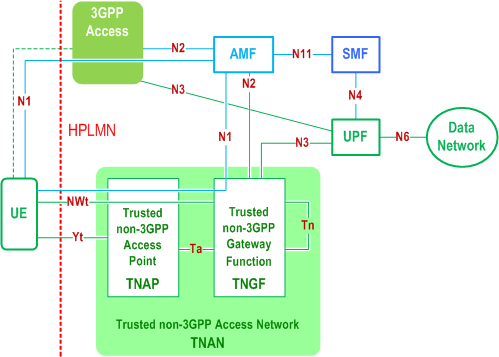
\includegraphics[width=0.5\linewidth]{figs/architecture-for-5g-core-network-with-trusted-non-3gpp-access.png}
    \caption{Architecture for 5G Core Network with Trusted Non-3GPP Access}
    \label{fig:architecture-for-5g-core-network-with-trusted-non-3gpp-access}
\end{figure}

\begin{figure}
    \centering
    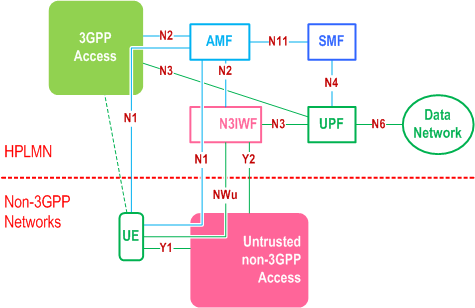
\includegraphics[width=0.5\linewidth]{figs/architecture-for-5g-core-network-with-untrusted-non-3gpp-access.png}
    \caption{Architecture for 5G Core Network with Untrusted Non-3GPP Access}
    \label{fig:architecture-for-5g-core-network-with-untrusted-non-3gpp-access}
\end{figure}

When using non-\ac{3GPP} access, UEs establish secure IPsec tunnels with the N3IWF or TNGF to register with the 5G Core Network. Post-registration, the NAS signaling between the UE and the core network is protected using the same security mechanisms as 3GPP access.

\begin{figure}
    \centering
    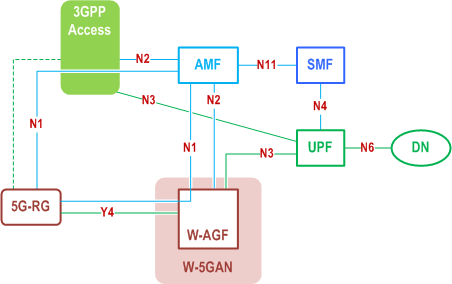
\includegraphics[width=0.5\linewidth]{figs/Architecture for 5G Core Network for 5G-RG with Wireline 5G Access network and NG RAN.png}
    \caption{Architecture for 5G Core Network for 5G-RG with Wireline 5G Access network and NG RAN}
    \label{fig:Architecture for 5G Core Network for 5G-RG with Wireline 5G Access network and NG RAN}
\end{figure}

Wireline 5G Access Networks (W-5GAN), such as broadband fiber-optic networks, connect to the 5G Core Network (5GC) via the Wireline Access Gateway Function (W-AGF) (see Figure \ref{fig:Architecture for 5G Core Network for 5G-RG with Wireline 5G Access network and NG RAN}), using N2 and N3 interfaces for control and user plane functions, respectively. When a 5G Residential Gateway (5G-RG), such as a home router with 5G capabilities, connects through both NG-RAN (Next Generation Radio Access Network, like a 5G cellular tower) and W-5GAN, it maintains separate N1 signaling instances for each access. However, a single AMF in the same 5G Core Network serves the 5G-RG. NAS signaling over W-5GAN persists even after PDU sessions are released or handed over to 3GPP access.

\subsection{Device Diversity and Access Options}

As the 5G network evolves, it's important to recognize that not all devices connected to the network are 5G capable. While we typically envision user equipment (UE) as being 5G-enabled, 3GPP has also accounted for a wide range of devices, from legacy systems to non-5G capable ones, ensuring that connectivity remains seamless and secure across diverse access points.

\begin{figure}
    \centering
    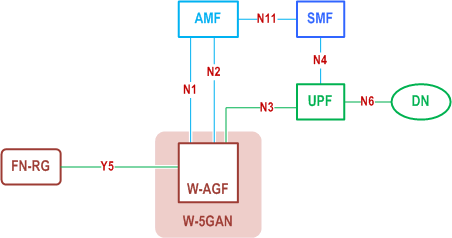
\includegraphics[width=0.5\linewidth]{figs/Architecture for 5G Core Network for FN-RG with Wireline 5G Access network and NG RAN.png}
    \caption{Architecture for 5G Core Network for FN-RG with Wireline 5G Access network and NG RAN}
    \label{fig:Architecture for 5G Core Network for FN-RG with Wireline 5G Access network and NG RAN}
\end{figure}

For non-5G-capable Fixed Network Residential Gateways (FN-RGs), such as legacy home routers, connected via W-5GAN (see Figure \ref{fig:Architecture for 5G Core Network for FN-RG with Wireline 5G Access network and NG RAN}), the W-AGF handles N1 signaling on behalf of the FN-RG. UEs, like smartphones or IoT devices, connecting through these gateways can access the 5G Core via either N3IWF (untrusted access using Wi-Fi) or TNGF (trusted access) depending on the network configuration.

\begin{figure}
    \centering
    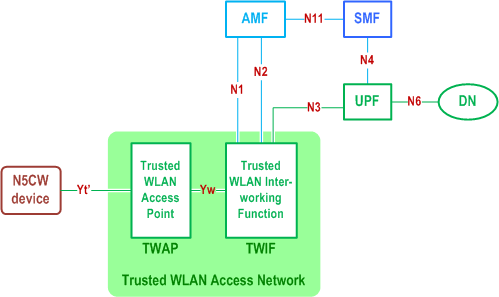
\includegraphics[width=0.5\linewidth]{figs/Architecture for supporting 5GC access from N5CW devices.png}
    \caption{Architecture for supporting 5GC access from N5CW devices}
    \label{fig:Architecture for supporting 5GC access from N5CW devices}
\end{figure}

There are also devices that are not 5G-capable over WLAN access, referred to as N5CW devices, cannot support 5GC NAS signaling over WLAN but may still operate as 5G UEs over NG-RAN. 3GPP provides enhancements for N5CW devices to access 5GC via trusted WLAN access networks (see Figure \ref{fig:Architecture for supporting 5GC access from N5CW devices}), which are a type of Trusted Non-3GPP Access Network (TNAN), typically using IEEE 802.11 technology. These networks must support specific functions, such as the Trusted WLAN Interworking Function (TWIF), which enables N5CW devices to register with the 5GC. When a N5CW device performs an EAP-based access authentication procedure to connect to a trusted WLAN access network, it may simultaneously be registered to a 5GC of a PLMN or SNPN. The TWIF handles authentication, AMF selection, NAS protocol communication, and relays user data between the WLAN access network and the 5GC. In this specification, trusted WLAN access for N5CW devices only supports IP PDU sessions.

\subsection{Authentication Flow Across Networks}
Examining the authentication flows for devices connecting to the 5G Core (5GC) via non-3GPP access networks reveals differences in the mechanisms used for trusted and untrusted accesses.

For untrusted non-3GPP access, security is established using IKEv2 to set up IPsec security associations between the UE (acting as the IKE initiator) and the N3IWF (acting as the IKE responder). The UE and N3IWF use a derived key from the AMF to complete the authentication process.

In non-roaming scenarios, the home operator (HPLMN) decides whether a non-3GPP access network is trusted or untrusted based on its security features, while in roaming scenarios, the decision is made by the UDM in the HPLMN. This decision applies consistently across all DNs the UE connects to via the same non-3GPP access network.

The UE stores trusted non-3GPP access network information in the USIM (Universal Subscriber Identity Module), which takes priority over the ME (Mobile Equipment), the device itself.

For authentication over untrusted non-3GPP networks (see Figure \ref{fig:Authentication for untrusted non-3GPP access}), the UE uses a vendor-specific EAP method called "EAP-5G," which employs the "Expanded" EAP type and the 3GPP Vendor-Id. The EAP-5G method is used between the UE and N3IWF to encapsulate NAS messages. If the UE requires authentication by the 3GPP home network, standard authentication methods are applied between the UE and the AUSF. Whenever possible, the UE will reuse the existing NAS security context from the AMF for authentication.
% cite 7.2.1 TS33.501

\begin{figure}
    \centering
    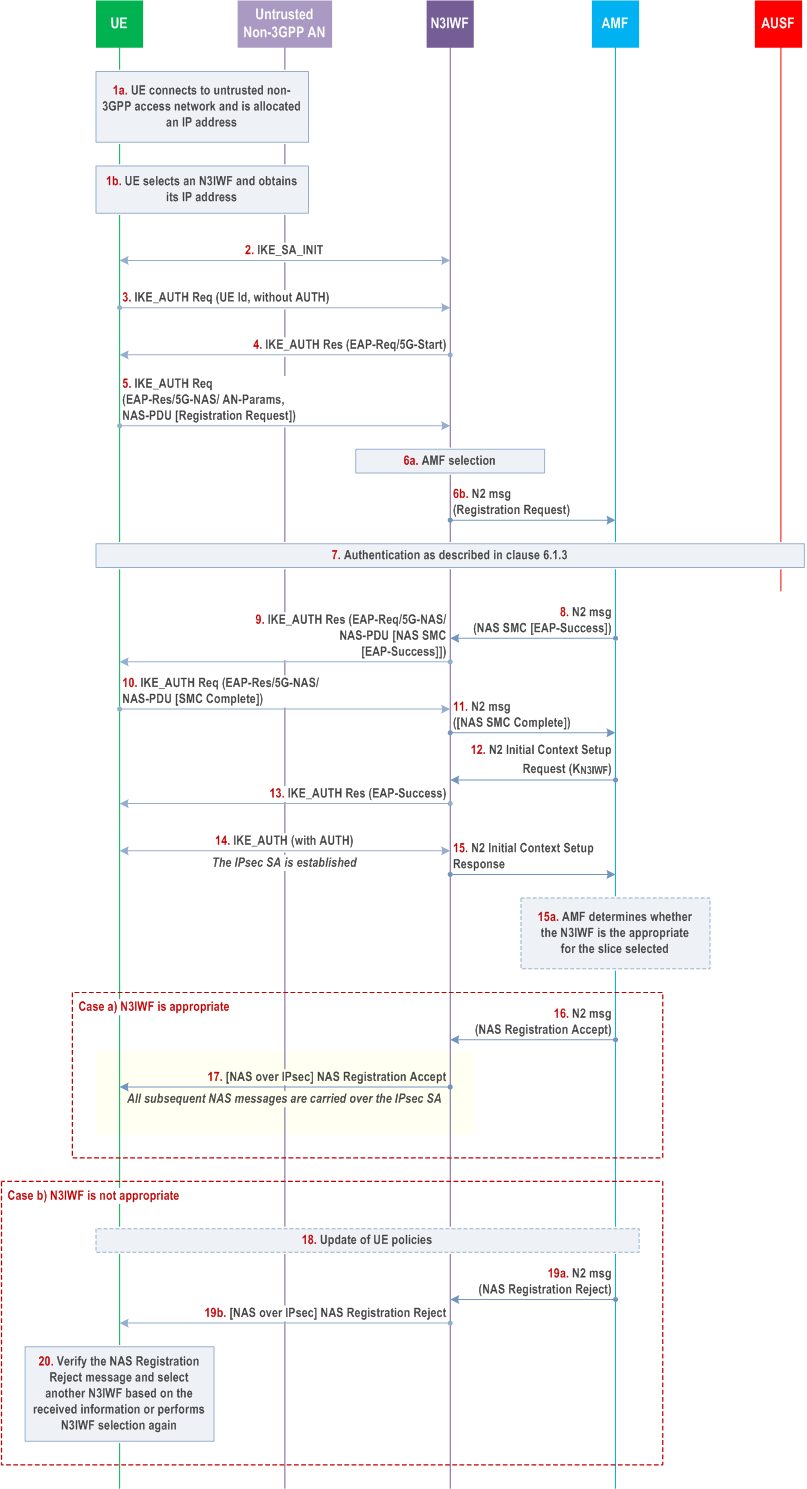
\includegraphics[width=0.75\linewidth]{figs/Authentication for untrusted non-3GPP access.png}
    \caption{Authentication for untrusted non-3GPP access}
    \label{fig:Authentication for untrusted non-3GPP access}
\end{figure}

Security for trusted non-3GPP access to the 5G Core (5GC) involves the UE registering to the 5GC via a Trusted Non-3GPP Access Network (TNAN) using the EAP-5G procedure, similar to that used for untrusted access (see Figure \ref{fig:Authentication and PDU Session establishment for trusted non-3GPP access_1}, \ref{fig:Authentication and PDU Session establishment for trusted non-3GPP access_2} and \ref{fig:Authentication and PDU Session establishment for trusted non-3GPP access_3} ). The link between the UE and the TNAN relies on Layer-2 security, making IPSec encryption unnecessary between the UE and the TNGF, though integrity protection is ensured.

During registration, the TNGF terminates EAP-5G signaling and forwards NAS messages to the 5GC. At the registration's conclusion, an IPSec SA (NWt) is established between the UE and TNGF to protect NAS messages. Additional IPSec SAs are created during PDU session establishment for user plane transport. Security policies, determined by the home operator, define whether non-3GPP access is trusted based on security domains or other considerations.

For trusted non-3GPP access authentication, key differences from untrusted access include avoiding IKEv2 encapsulation for EAP-5G packets, utilizing 5G-GUTI or SUCI for UE identity, and deriving keys like $K_TNGF$ and $K_TNAP$ for secure communication. These keys are shared between the AMF, TNGF, and TNAP to establish secure communication flows.

\begin{figure}
    \centering
    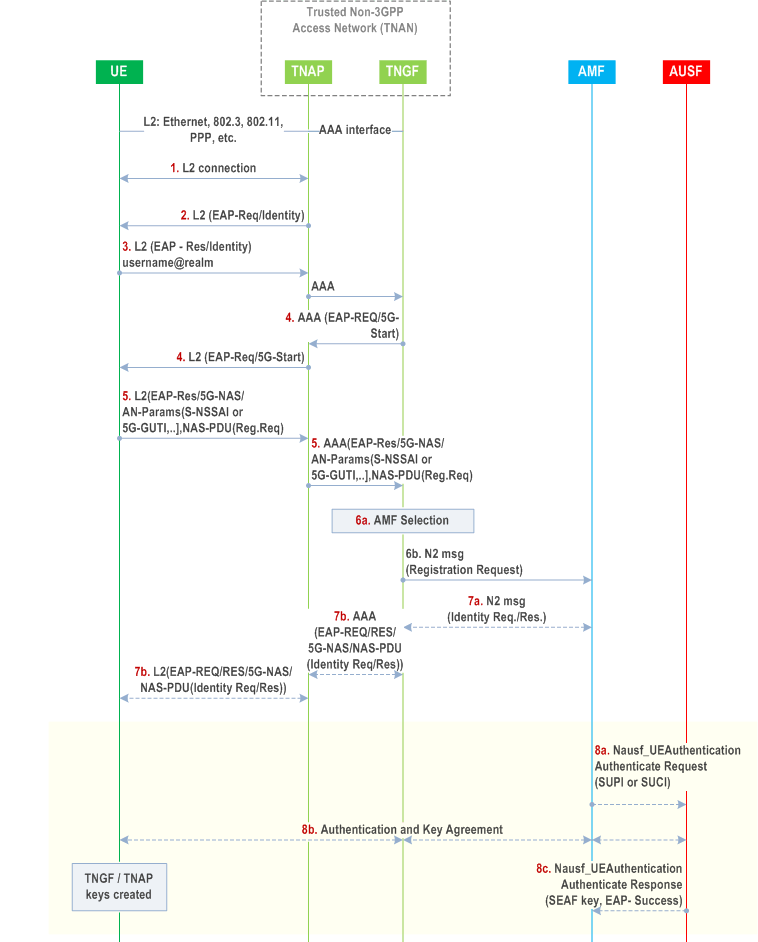
\includegraphics[width=0.75\linewidth]{figs/Authentication and PDU Session establishment for trusted non-3GPP access_1.png}
    \caption{Authentication and PDU Session establishment for trusted non-3GPP access}
    \label{fig:Authentication and PDU Session establishment for trusted non-3GPP access_1}
\end{figure}

\begin{figure}
    \centering
    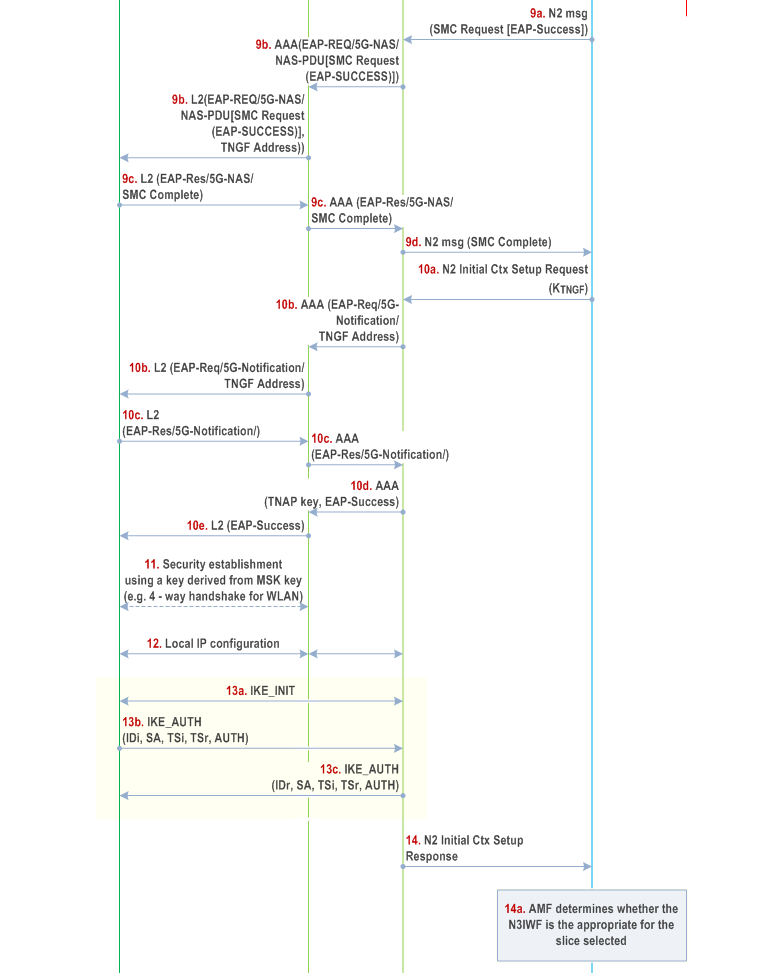
\includegraphics[width=0.75\linewidth]{figs/Authentication and PDU Session establishment for trusted non-3GPP access_2.png}
    \caption{Authentication and PDU Session establishment for trusted non-3GPP access (continuation)}
    \label{fig:Authentication and PDU Session establishment for trusted non-3GPP access_2}
\end{figure}

\begin{figure}
    \centering
    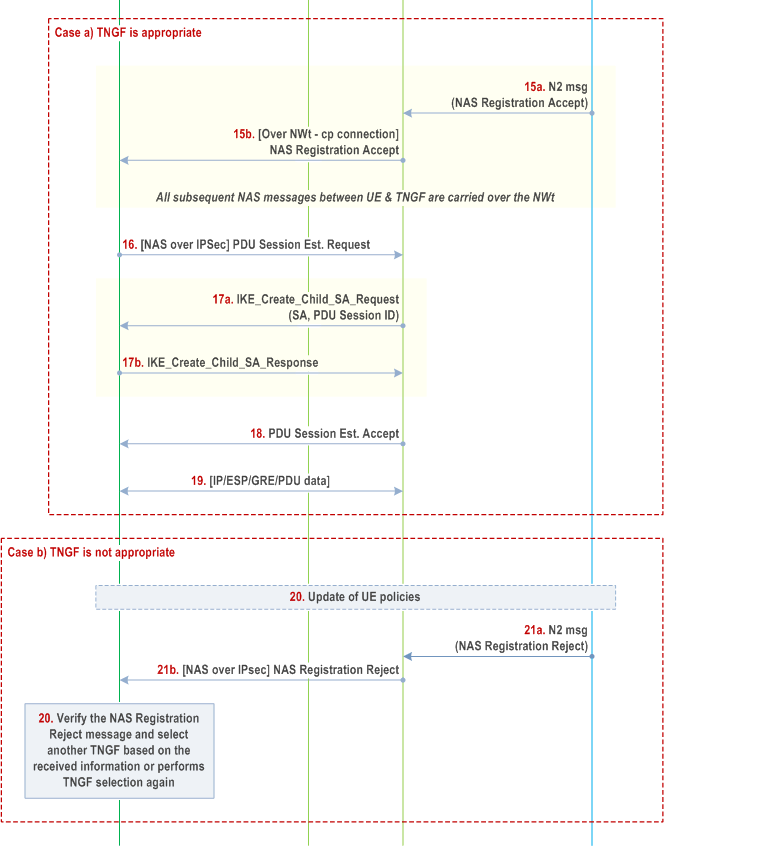
\includegraphics[width=0.75\linewidth]{figs/Authentication and PDU Session establishment for trusted non-3GPP access_3.png}
    \caption{Authentication and PDU Session establishment for trusted non-3GPP access (continuation)}
    \label{fig:Authentication and PDU Session establishment for trusted non-3GPP access_3}
\end{figure}

To support the integration of wireless and wireline technologies in the 5G system, two new network entities, the 5G-RG and FN-RG, connect to the 5G Core (5GC) via a wireline access network (W-5GAN) or Fixed Wireless Access (FWA). Both entities ensure that non-5G capable devices, such as laptops and IoT devices, behind them can connect to the 5GC. The 5G-RG handles NAS signaling itself, while the FN-RG relies on the W-AGF (Wireline Access Gateway Function) for registration and signaling. The same 5G security procedures apply to both setups, ensuring consistency across wireless and wireline access.

For example, in a smart home, devices could connect to the 5GC through a 5G-RG using fiber or FWA. Similarly, in an enterprise environment, an FN-RG could provide secure, high-speed access via wireline networks. The link between the RG and W-5GAN leverages 5G’s security framework to protect the connection, similar to wireless setups. However, roaming is not supported for these entities or the devices they serve. Additional EAP methods may be applied in isolated setups, as we will discuss next, to ensure secure authentication for devices in unique configurations. For instance, a remote workstation connected via wireline can still securely access the 5GC. This approach enables secure, seamless convergence of 5G across both fixed and wireless network environments.

The 5G-RG supports connections to the 5GC via NG-RAN, W-5GAN, or both. Its registration processes depend on the access type. When connecting through NG-RAN, the procedure follows TS 23.316 clause 4.11, while W-5GAN connections adhere to clause 7.2.1, leveraging the untrusted non-3GPP access method. As the 5G-RG is equivalent to a UE from the 5GC’s viewpoint, it utilizes the standard authentication framework, including 5G-AKA and EAP-AKA’. For W-5GAN connections, W-CP protocol stack messages are used to encapsulate NAS signaling.

In contrast, the FN-RG connects solely via W-5GAN and relies on the W-AGF to manage N1 signaling on its behalf, as it does not inherently support N1. The W-AGF provides connectivity to the 5GC through N2 and N3 interfaces and can authenticate the FN-RG based on local policies. A mutual trust relationship between the wireline operator managing the W-5GAN and the PLMN operator managing the 5GC is established using secure protocols like NDS/IP or DTLS.

\section{Device Support Behind Wireline}

So far we have explored how 3GPP and non-3GPP access types—trusted, untrusted, and wireline—enable diverse devices to connect to the 5G Core (5GC). While trusted and untrusted non-3GPP access methods typically require user equipment (UE) to possess full 5G capabilities, including NAS signaling and the ability to derive the 5G key hierarchy, wireline access uniquely bridges the gap for devices lacking these capabilities.
% cite Annex O ts 33.501 regarding  key derivation

It's important to note that some devices, such as Non-5G-Capable over WLAN (N5CW) devices, occupy a middle ground. Despite lacking full 5G functionality over WLAN, N5CW devices can still register with the 5GC, establish PDU sessions, and utilize 3GPP credentials (USIM) for authentication. They may even function as regular 5G UEs when connected via cellular networks. This contrasts with Non-5G Capable (N5GC) devices, which lack these 5G-specific capabilities entirely.

Unlike wireless access, which assumes RAN functionality within the device, wireline access leverages network entities such as the FN-RG and 5G-RG to facilitate connectivity. These gateways act on behalf of the devices, ensuring secure access to the 5GC even for non-5G-capable devices in wireline environments. For instance, the W-AGF (Wireline Access Gateway Function) can perform UE registration procedures on behalf of an FN-RG, bridging the gap for devices that cannot handle NAS signaling themselves.

This approach enables a wide range of devices, from IoT sensors to legacy equipment, to benefit from 5G connectivity without requiring full 5G capabilities. The flexibility to support diverse device types and access methods, including those with partial 5G capabilities like N5CW devices, highlights the critical role of wireline access in achieving seamless 5G convergence across both fixed and wireless network environments.

Given that N5GC devices lack the capability to derive 5G keys and perform other UE-expected procedures, the W-AGF must handle additional responsibilities, including managing device identifiers. For N5GC devices connecting via CRG, the SUPI contains a network-specific identifier in the form of a Network Access Identifier (NAI). The W-AGF plays a crucial role in deriving the SUCI from the EAP-Identity message received from the N5GC device and providing it to the AMF. This SUCI, formatted according to TS 23.003, serves as a secure identifier for the N5GC device within the 5G system. By handling these identifier-related tasks, the W-AGF effectively bridges the gap between N5GC devices and the 5G Core, enabling their integration into the 5G ecosystem despite their limited capabilities
%cite 23.316 4.7.11 untill here!

\subsection{5GC Registration Process for N5GC Devices}

In isolated 5G networks with wireline access, non-5G-capable (N5GC) devices can access the 5G Core (5GC) through a structured process involving EAP-based authentication. Each N5GC device is treated as an individual entity with its own subscription record in the UDM/UDR, distinct from the subscription record of the Customer Residential Gateway (CRG). The CRG operates in L2 bridge mode, forwarding traffic from connected N5GC devices to the Wireline Access Gateway Function (W-AGF) for further processing and registration.

\begin{figure}
    \centering
    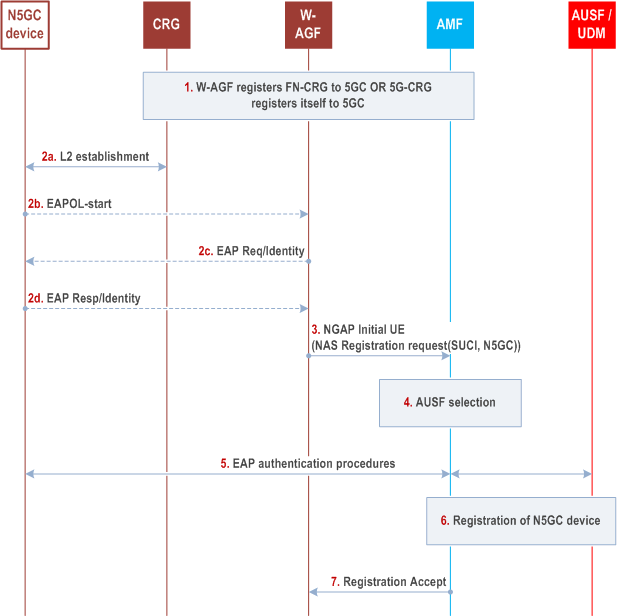
\includegraphics[width=0.75\linewidth]{figs/5GC registration of Non-5GC device.png}
    \caption{5GC registration of Non-5GC device}
    \label{fig:5GC registration of Non-5GC device}
\end{figure}

The process begins with the registration of the CRG to the 5GC (the flow is shown in Figure \ref{fig:5GC registration of Non-5GC device}). This enables the CRG to act as a bridge, facilitating communication between N5GC devices and the W-AGF. Once this setup is in place, authentication is triggered when the CRG forwards traffic from an N5GC device. This occurs either through the reception of an EAPOL-Start frame sent by the N5GC device or when the W-AGF detects traffic from an unknown MAC address. The N5GC device responds by sending an EAP-Response/Identity message containing its Network Access Identifier (NAI), formatted as \texttt{username@realm}.

The W-AGF then acts on behalf of the N5GC device to initiate its registration with the 5GC. It constructs and sends a NAS Registration Request to the AMF, including a SUCI derived from the NAI. This registration explicitly indicates that the device lacks native 5G capabilities. The W-AGF establishes separate NGAP connections for each N5GC device over the N2 interface, enabling distinct communication channels for every device.

Authentication of the N5GC device is carried out by the AUSF using EAP-based methods. Once the device successfully authenticates, the AUSF provides the relevant security information to the AMF, including the SUPI derived from the NAI. This SUPI uniquely identifies the N5GC device within the 5GC ecosystem, ensuring individual accountability and secure operation.

Following successful authentication, the AMF completes additional registration procedures. If a PEI is required, the W-AGF uses the MAC address of the N5GC device, with an option to encode it in IEEE EUI-64 format depending on operator policy. Once registration is finalized, the W-AGF communicates the Registration Accept message to the N5GC device, marking the completion of the process.

After registration, the W-AGF establishes a single PDU session for each N5GC device, ensuring each device is assigned its own unique data session within the 5GC while accounting for the device's limitations. This ensures secure and individualized connectivity. Additionally, the W-AGF manages NGAP connections, ensuring that if the NGAP connection for a CRG is released, all associated N5GC device connections are also terminated. The CRG continues to operate as an FN-CRG, supporting seamless communication for connected devices.
%cite 23.316 4.10a for paragraphs until here!!

\begin{figure}
    \centering
    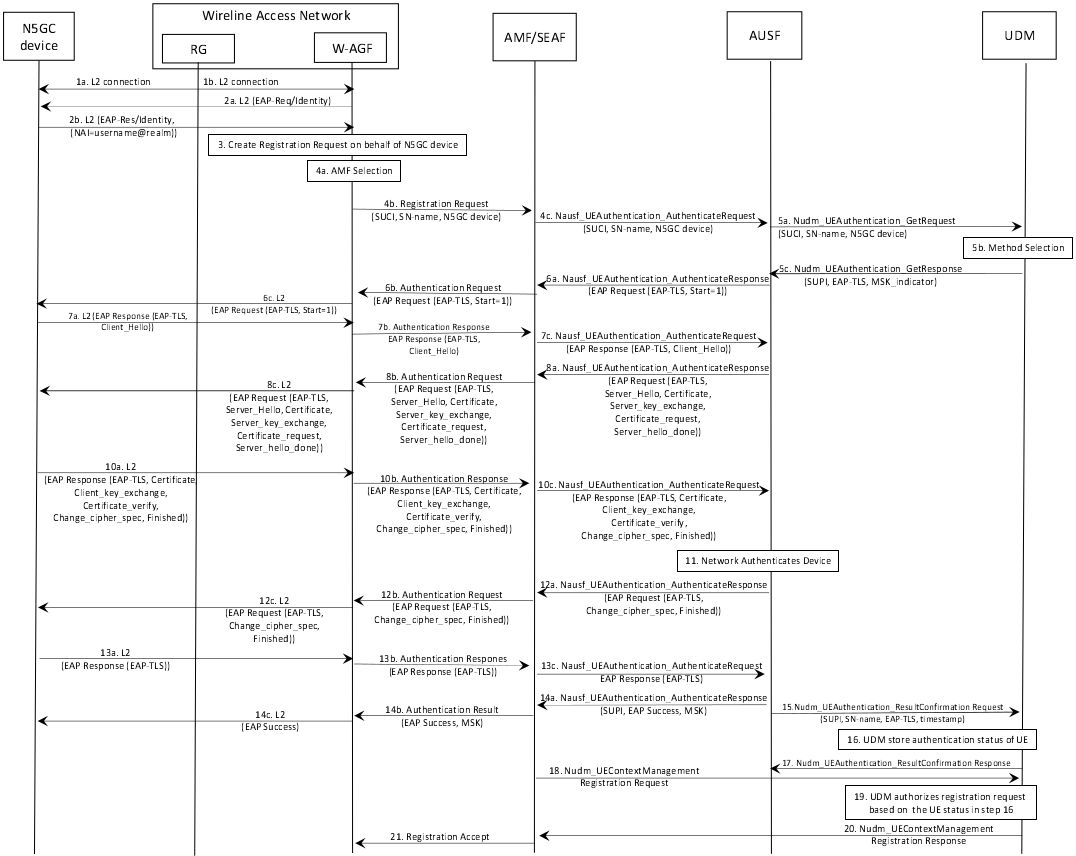
\includegraphics[width=0.75\linewidth]{figs/Detailed registration and authentication flow of a non-5G capable device to the 5GC.png}
    \caption{Detailed registration and authentication flow of a non-5G capable device to the 5GC}
    \label{fig:Detailed registration and authentication flow of a non-5G capable device to the 5GC}
\end{figure}

In Annex 0 of TS 33.501, we can get more detail regarding this registration and authentication process (see Firgure \ref{fig:Detailed registration and authentication flow of a non-5G capable device to the 5GC}).
% Annex O 33.501

\subsection{Non-5G-capable (N5GC) and Non-Authenticable Non-3GPP (NAUN3) devices}

A Non-Authenticable Non-3GPP (NAUN3) device does not support NAS signalling, is connected to 5GC via a RG and does not support authentication with the 5GC.%cite TS 23.316 3.1

NAUN3 devices, which cannot be authenticated by the 5GC, may be locally authenticated by the 5G-RG using methods like pre-shared secrets. Examples of pre-shared secrets include Wi-Fi passphrases for SSIDs, PIN codes, or static security keys configured during device setup. Differentiated services, including Quality of Service (QoS) and network slicing, can be applied to these devices through "Connectivity Group IDs" (CGIDs) (see Figure \ref{fig:NAUN3 devices behind 5G-RG based on connectivity groups}).

\begin{figure}
    \centering
    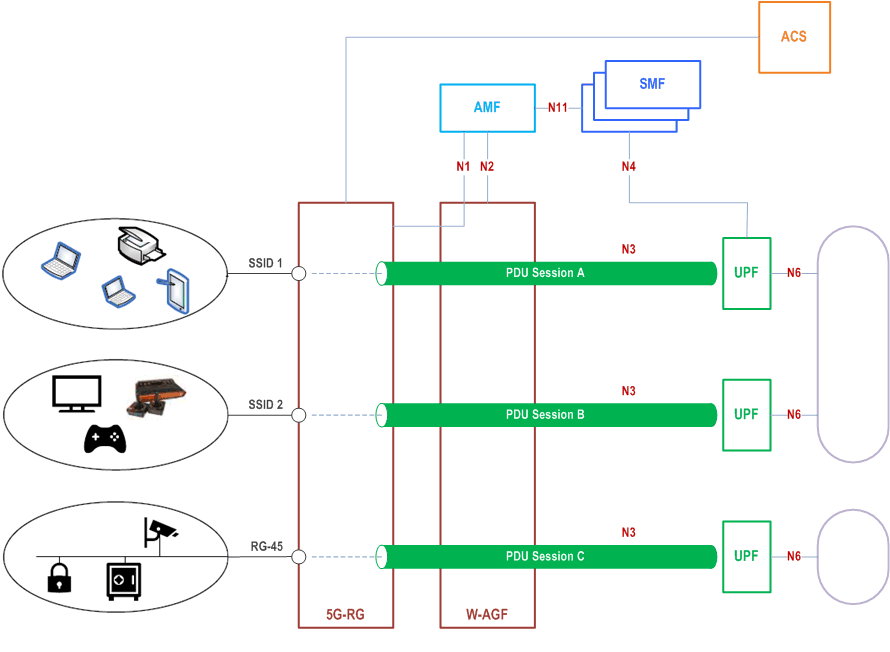
\includegraphics[width=0.75\linewidth]{figs/NAUN3 devices behind 5G-RG based on connectivity groups.png}
    \caption{NAUN3 devices behind 5G-RG based on connectivity groups}
    \label{fig:NAUN3 devices behind 5G-RG based on connectivity groups}
\end{figure}

Each CGID corresponds to a specific physical or virtual port on the 5G-RG, such as Ethernet ports, WLAN SSIDs, or VLANs. Devices connected to the same logical port are considered part of the same CGID, and each CGID maps to a separate PDU (Protocol Data Unit) Session established by the 5G-RG to manage their traffic.

The 5G-RG is configured with port information, such as VLANs and SSIDs, via standardized protocols like TR-69, TR-360, and TR-181. URSP (User Equipment Route Selection Policy) rules are provided to the 5G-RG to define how CGIDs are mapped to PDU Session parameters, such as the DNN (Data Network Name) and S-NSSAI (Single Network Slice Selection Assistance Information). These mappings determine how traffic is routed and which network slice the devices use. For instance, a home office CGID might map to a DNN providing enterprise services and an S-NSSAI prioritizing low latency for work-related tasks.

Charging and QoS differentiation for NAUN3 devices can be implemented through PCC (Policy and Charging Control) rules. These rules define service flows tied to specific PDU Sessions, enabling detailed traffic management and billing policies. Additionally, isolation of devices using a specific CGID into a separate network slice (associated with an S-NSSAI) can provide enhanced security and service customization. For example, devices in a child’s CGID could be isolated into a network slice with strict content filtering and bandwidth limitations. However, configuration specifics for connecting NAUN3 devices to particular ports or SSIDs remain outside the scope of this specification.%cite 23.316 4.10b

The main difference between NAUN3 and N5GC devices lies in their capabilities and how they interact with the 5G Core (5GC), here is a summary of what we've seen soo far:

\begin{itemize}
    \item {
        \textbf{NAUN3 Devices}
        \begin{itemize}
            \item {
                \textbf{Authentication}: They cannot be authenticated by the 5GC. Instead, they rely on local authentication mechanisms provided by the 5G-RG (e.g., Wi-Fi passphrases, PINs, or pre-shared keys).
            }
            \item {
                \textbf{Connection}: NAUN3 devices connect through the 5G-RG, which maps their traffic to PDU Sessions (Protocol Data Unit Sessions) and handles aspects like Quality of Service (QoS) and network slicing (e.g., via S-NSSAI, Single Network Slice Selection Assistance Information).
            }
            \item {
                \textbf{Subscription Records}: NAUN3 devices do not have subscription records in the 5G Core and operate entirely under the configuration and policies of the 5G-RG.
            }
            \item {
                \textbf{Purpose}: They are typically legacy or IoT devices that do not need direct 5GC access but require differentiated services provided via local configuration and mapping.
            }
            \item {
                \textbf{Example}: A smart home appliance connected to the 5G-RG via Wi-Fi using a pre-shared key, with its traffic routed through a dedicated network slice.
            }
        \end{itemize}    
    }
    \item {
        \textbf{N5GC Devices}
        \begin{itemize}
            \item {
                \textbf{Authentication}: They can be authenticated by the 5GC using EAP-based authentication (Extensible Authentication Protocol) with the help of the W-AGF (Wireline Access Gateway Function), which acts as an intermediary.
            }
            \item {
                \textbf{Connection}: N5GC devices connect to the 5GC through wireline access (e.g., fiber or DSL) and use the W-AGF to handle their registration, authentication, and session management.
            }
            \item {
                \textbf{Subscription Records}: Each N5GC device has its own unique subscription record in the UDM/UDR (Unified Data Management/Unified Data Repository), separate from the subscription record of the CRG (Customer Residential Gateway).
            }
            \item {
                \textbf{NGAP Connections}: The W-AGF establishes separate NGAP (Next Generation Access Protocol) connections for each N5GC device over the N2 interface to the AMF (Access and Mobility Management Function). This enables individual session and mobility management for each device.
            }
            \item {
                \textbf{Purpose}: N5GC devices extend 5G Core services to fixed network devices that do not possess 5G capabilities.
            }
            \item {
                \textbf{Example}: A desktop computer connected to the 5GC via fiber access and authenticated using EAP over the W-AGF.
            }
        \end{itemize}    
    }
\end{itemize}

\begin{table}[ht]
    \centering
    \caption{Key Differences between NAUN3 and N5GC devices}
    \label{tab:Key Differences between NAUN3 and N5GC devices}
    \begin{tabularx}{\textwidth} { 
      | >{\raggedright\arraybackslash}X 
      | >{\raggedright\arraybackslash}X 
      | >{\raggedright\arraybackslash}X | }
        \hline
        \textbf{Feature} & \textbf{NAUN3 Devices} & \textbf{N5GC Devices} \\
        \hline
        \textbf{5G Capability} & No 5G capability, cannot access 5GC directly. & Limited 5G capability, requires assistance to connect to 5GC.\\
        \hline
        \textbf{Authentication} & Local (e.g., Wi-Fi passphrase, PIN). & 5GC authentication via EAP and W-AGF.\\
        \hline
        \textbf{Access Type} & Wireless (e.g., Wi-Fi via 5G-RG). & Wireline (e.g., fiber via W-AGF).\\
        \hline
        \textbf{Subscription Records} & None in UDM/UDR; operates under 5G-RG policies. & Unique subscription records separate from CRG.\\
        \hline
        \textbf{NGAP Connections} & Not applicable. & Separate NGAP connections per device.\\
        \hline
        \textbf{Session Handling} & Handled by the 5G-RG. & Handled by W-AGF and 5GC.\\
        \hline
        \textbf{Purpose} & Legacy IoT or low-capability devices. & Wireline devices requiring 5GC services.\\
        \hline
        \textbf{Example} & Smart home appliance using Wi-Fi. & Desktop computer on a fiber network.\\
        \hline
    \end{tabularx}
\end{table}

In summary, NAUN3 devices operate entirely locally, with no interaction with the 5G Core, while N5GC devices leverage intermediaries like the W-AGF to authenticate and establish PDU Sessions with the 5GC, maintaining unique subscription records and dedicated NGAP connections.

%%%%%% REVIEWED SOO FAR !!! %%%%%%

\section{Wi-Fi-only Devices Integration Challenges}

\section{Current Solutions and Proposals}'